%!TEX root = ../template.tex
%%%%%%%%%%%%%%%%%%%%%%%%%%%%%%%%%%%%%%%%%%%%%%%%%%%%%%%%%%%%%%%%%%%%
%% chapter4.tex
%% NOVA thesis document file
%%
%% Chapter with lots of dummy text
%%%%%%%%%%%%%%%%%%%%%%%%%%%%%%%%%%%%%%%%%%%%%%%%%%%%%%%%%%%%%%%%%%%%

\typeout{NT FILE chapter4.tex}%

\chapter{Algoritmi Euristici e Metaeuristici}\label{chapt:4}
\section{Approcci Euristici}

Gli approcci euristici per risolvere problemi come il \gls{TSP} sono strategie progettate per trovare soluzioni sufficientemente buone entro un tempo ragionevole, specialmente quando una soluzione esatta non è fattibile a causa della complessità \cite{Johnson2002} del problema. Questi metodi sono essenziali nei casi in cui il costo computazionale per trovare la soluzione ottimale è proibitivo, come è comune con i problemi NP-difficili come il \gls{TSP} \cite{Cormen2009}.

\subsection{Concetto e Necessità}
Il concetto di approcci euristici si basa sull'idea di fare ipotesi educate o seguire algoritmi intuitivi che mirano a trovare soluzioni che siano vicine al miglior possibile, senza necessariamente garantire l'ottimalità \cite{Papadimitriou1998}. Le euristiche sono caratterizzate dalle loro strategie empiriche che le rendono significativamente più veloci rispetto ai metodi esatti nella pratica, sebbene a costo di potenzialmente perdere la soluzione ottimale.

La necessità delle euristiche deriva dall'intrattabilità computazionale di molti problemi del mondo reale \cite{Lawler1985}. Per il \gls{TSP}, man mano che il numero di città aumenta, lo spazio di ricerca (cioè, il numero totale di possibili tour) cresce in modo fattoriale, rendendo impossibile esplorare ogni opzione direttamente attraverso metodi di forza bruta in un intervallo di tempo ragionevole\cite{Gutin2016}. Le euristiche offrono un'alternativa pragmatica fornendo soluzioni che, pur non essendo garantite come ottimali, sono sufficientemente accurate per scopi pratici e possono essere ottenute molto più rapidamente \cite{Aarts1989}.

\subsection{Algoritmi Greedy}

Gli algoritmi greedy costituiscono una classe significativa di approcci euristici caratterizzati dalla loro strategia di fare la scelta localmente ottimale in ogni fase con la speranza di trovare un ottimo globale \cite{Cormen2009}. Nel contesto del \gls{TSP} e di problemi di ottimizzazione simili, gli algoritmi greedy semplificano i processi decisionali suddividendo un problema in una serie di passaggi e scegliendo la migliore opzione disponibile in ogni passaggio senza considerare le conseguenze più ampie di queste scelte\cite{Johnson2002}.

\subsubsection{Definizione e Principio}

Un algoritmo greedy costruisce una soluzione pezzo per pezzo, scegliendo sempre il pezzo successivo che offre il beneficio più immediato\cite{Papadimitriou1998}. Questo approccio è semplice e diretto, rendendolo un'opzione attraente per molti problemi in cui una soluzione rapida e facile è più preziosa di una ottimale. L'efficacia degli algoritmi greedy varia ampiamente da un problema all'altro; in alcuni casi, raggiungono una soluzione ottimale, mentre in altri, possono raggiungere solo una soluzione subottimale\cite{Lawler1985}.

\subsubsection{Applicazione al \gls{TSP}: Nearest Neighbor Search}

Nel \gls{TSP}, un'applicazione classica dell'algoritmo greedy è il Nearest Neighbor Search \gls{NNS}, dove l'algoritmo costruisce un tour partendo da una città arbitraria e, ad ogni passo, estende il tour spostandosi verso la città non visitata più vicina fino a quando tutte le città sono visitate\cite{Gutin2016}.


\newcommand{\tspnearestneighbor}[1]{%
	\begin{figure}[htbp]
		\centering
		\foreach \step in {1,...,5}{%
				\begin{subfigure}[b]{0.33\textwidth} % Adjust the width for 2 columns
					\centering
					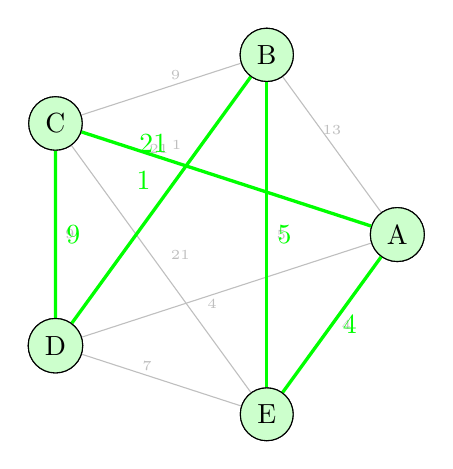
\begin{tikzpicture}[scale=0.8]
						% Define nodes
						\node[circle,draw,fill=green!20] (A) at (1 * 3,0) {A};
						\node[circle,draw] (B) at (0.309 * 3,0.951 * 3) {B};
						\node[circle,draw] (C) at (-0.809*3,0.588*3) {C};
						\node[circle,draw] (D) at (-0.809*3,-0.588*3) {D};
						\node[circle,draw] (E) at (0.309*3,-0.951*3) {E};

						% Draw all edges in light gray
						\ifthenelse{\step < 5}{%
							\draw[lightgray] (A) -- node[above] {\tiny 13} (B);
							\draw[lightgray] (A) -- node[below left] {\tiny 4} (D);
							\draw[lightgray] (A) -- node[pos = 2/3, above left] {\tiny 21} (C);
							\ifthenelse{\step < 1}{\draw[lightgray] (A) -- node[right] {\tiny 4} (E);}{}
							\draw[lightgray] (B) -- node[above right] {\tiny 9} (C);
							\ifthenelse{\step < 2}{\draw[lightgray] (B) -- node[right] {\tiny 5} (E);}{}

							\ifthenelse{\step < 4}{
								\draw[lightgray] (C) -- node[above right] {\tiny 21} (E);
								\draw[lightgray] (C) -- node[right] {\tiny 9} (D);}{}
							\draw[lightgray] (D) -- node[pos = 1/2, above left] {\tiny 7} (E);
							\ifthenelse{\step < 3}{\draw[lightgray] (B) -- node[pos = 1/3, above left] {\tiny 1} (D);}{}
						}{}

						% Highlight the path based on the step
						\ifthenelse{\step > 0}{%
							\draw[green,very thick] (A) -- node[right] {4} (E);
							\node[circle,fill=green!20,draw] at (A) {A};
						}{}
						\ifthenelse{\step > 1}{%
							\draw[green,very thick] (E) -- node[right] {5} (B);
							\node[circle,fill=green!20,draw] at (E) {E};
						}{}
						\ifthenelse{\step > 2}{%
							\draw[green,very thick] (B) -- node[above left] {1} (D);
							\node[circle,fill=green!20,draw] at (B) {B};
						}{} 		
						\ifthenelse{\step > 3}{%
							\draw[green,very thick] (D) -- node[right] {9} (C);
							\node[circle,fill=green!20,draw] at (D) {D};
						}{}
						\ifthenelse{\step > 4}{%
							\draw[green,very thick] (C) -- node[pos = 1/3, above left] {21} (A);
							\node[circle,fill=green!20,draw] at (C) {C};
						}{}
					\end{tikzpicture}
					\caption{Iterazione \step}
				\end{subfigure}%
				\ifnum\step>0
					\ifnum\numexpr\step+1\relax=3\relax
						\par\vspace{\baselineskip}
					\fi
				\fi
			}%
	\end{figure}
}


\tspnearestneighbor{6}
\paragraph{Pseudocodice}

\begin{algorithm}
	\caption{TSP \gls{NNS}}\label{alg:greedybestfirst}
	\begin{algorithmic}[1]
		\Procedure{NearestNeighborSearch}{$cities, distances$}
		\State $start \gets$ seleziona una città arbitraria da $cities$
		\State $current \gets start$
		\State $tour \gets$ lista contenente $start$
		\State $unvisited \gets cities \setminus \{start\}$
		\While{$unvisited \neq \emptyset$}
		\State $next \gets$ città in $unvisited$ con distanza minima da $current$
		\State aggiungi $next$ a $tour$
		\State rimuovi $next$ da $unvisited$
		\State $current \gets next$
		\EndWhile
		\State aggiungi $start$ a $tour$ per chiudere il ciclo
		\State \Return $tour$
		\EndProcedure
	\end{algorithmic}
\end{algorithm}

Questa strategia greedy assicura che ad ogni passo, il tour cresca aggiungendo la destinazione più vicina possibile, ottimizzando per il passo immediato successivo senza considerare la lunghezza complessiva del tour. Sebbene questo metodo non garantisca la scoperta del tour più breve possibile, riduce significativamente il tempo di calcolo rispetto ai metodi di ricerca esaustiva.

% TODO: Riordina questo

\subsubsection{Vantaggi e Limitazioni}

\textbf{Vantaggi:}
\begin{itemize}
	\item \textit{Semplicità}: Gli algoritmi greedy sono semplici da implementare e comprendere.
	\item \textit{Efficienza}: Spesso forniscono soluzioni rapidamente, rendendoli adatti per problemi in cui la velocità è cruciale.
\end{itemize}

\textbf{Limitazioni:}
\begin{itemize}
	\item \textit{Ottimalità}: Le scelte greedy non portano sempre alla soluzione ottimale, specialmente per problemi complessi come il \gls{TSP}.
	\item \textit{Corto raggio di azione}: Concentrandosi sull'ottimalità locale, potrebbero trascurare soluzioni migliori che richiedono scelte iniziali non ottimali.
\end{itemize}

Gli algoritmi greedy, con la loro semplicità ed efficienza intrinseche, giocano un ruolo cruciale nella risoluzione euristica dei problemi, specialmente nei casi in cui ottenere una soluzione esatta è computazionalmente impraticabile. La loro applicazione al \gls{TSP} evidenzia l'equilibrio tra efficienza computazionale e qualità della soluzione, un tema che risuona attraverso lo studio degli algoritmi euristici e metaeuristici.

\section{Algoritmi di Local Search}

Gli algoritmi di ricerca locale rappresentano una classe di metodi euristici progettati per esplorare lo spazio delle soluzioni di un problema di ottimizzazione spostandosi iterativamente da una soluzione a una soluzione vicina nello spazio di ricerca. Questi algoritmi sono particolarmente efficaci per problemi come il \gls{TSP}, dove trovare una soluzione ottimale è computazionalmente impraticabile per istanze grandi. La ricerca locale fornisce un meccanismo per migliorare una soluzione iniziale attraverso piccole modifiche localizzate \cite{Johnson2002,Lawler1985}.

\subsection{Tecniche 2-opt e 3-opt}

Le tecniche 2-opt e 3-opt sono strategie di ricerca locale specifiche utilizzate per affinare le soluzioni del \gls{TSP}. Funzionano rimuovendo iterativamente due o tre archi dal tour e riconnettendo i segmenti in un ordine diverso, mirando a ridurre la lunghezza totale del tour con ogni operazione.

\subsubsection{Tecnica 2-opt}

L'algoritmo 2-opt controlla sistematicamente ogni coppia di archi nel tour e determina se lo scambio di essi porterebbe a un percorso più breve. Questo processo viene ripetuto fino a quando non possono essere apportati ulteriori miglioramenti.


\begin{center}
	\begin{figure}[h]
		\caption{Scambio 2-opt}
		\begin{tikzpicture}
			% Definisci i nodi
			\node[draw=none, fill=none] (A) at (0,2) {A};
			\node[draw=none] (B) at (2,1.7) {B};
			\node[draw=none] (C) at (4,1.5) {C};
			\node[draw=none] (D) at (6,2) {D};

			\node[draw=none] (G) at (0,0) {G};
			\node[draw=none] (F) at (2,0.2) {F};
			\node[draw=none] (E) at (4,0.5) {E};

			% Collega i nodi
			\draw (A) -- (B);
			\draw[red] (B) -- (E);
			\draw (E) -- (D);
			\draw (D) -- (C);
			\draw[red] (C) -- (F);
			\draw (F) -- (G);
			\draw (G) -- (A);

			% Definisci i nodi
			\node[draw=none] (A2) at (10-2,2) {A};
			\node[draw=none] (B2) at (12-2,1.7) {B};
			\node[draw=none] (C2) at (14-2,1.5) {C};
			\node[draw=none] (D2) at (16-2,2) {D};

			\node[draw=none] (G2) at (10-2,0) {G};
			\node[draw=none] (F2) at (12-2,0.2) {F};
			\node[draw=none] (E2) at (14-2,0.5) {E};

			% Collega i nodi
			\draw (A2) -- (B2);
			\draw[blue] (B2) -- (C2);
			\draw (E2) -- (D2);
			\draw (D2) -- (C2);
			\draw[blue] (E2) -- (F2);
			\draw (F2) -- (G2);
			\draw (G2) -- (A2);
		\end{tikzpicture}
	\end{figure}
\end{center}

\begin{algorithm}
	\caption{Tecnica 2-opt per \gls{TSP}}\label{alg:twoopt}
	\begin{algorithmic}[1]
		\Procedure{TwoOpt}{$tour, distances$}
		\State $improved \gets true$
		\While{$improved$}
		\State $improved \gets false$
		\For{$i \gets 1$ to length($tour$) - 1}
		\For{$j \gets i+1$ to length($tour$)}
		\If{\Call{TwoOptSwap}{$tour, i, j$} $<$ \Call{TourDistance}{$tour$}}
		\State $tour \gets$ \Call{TwoOptSwap}{$tour, i, j$}
		\State $improved \gets true$
		\EndIf
		\EndFor
		\EndFor
		\EndWhile
		\State \Return $tour$
		\EndProcedure
	\end{algorithmic}
\end{algorithm}

\subsubsection{Tecnica 3-opt}

La tecnica 3-opt estende l'idea del 2-opt considerando tre archi per la riconnessione. Questo consente una gamma più ampia di riarrangiamenti ad ogni passo, potenzialmente portando a miglioramenti più significativi a scapito di una maggiore complessità computazionale.

\paragraph{Pseudocodice per la Tecnica 3-opt} è concettualmente simile al 2-opt ma coinvolge più condizioni per gli scambi, riflettendo la maggiore complessità di considerare tre archi alla volta.

\subsection{Lin–Kernighan}

L'algoritmo di Lin-Kernighan (\gls{LK}) è una delle tecniche più avanzate e potenti di ricerca locale per risolvere il \gls{TSP}. Proposto da Shen Lin e Brian W. Kernighan nel 1973, questo algoritmo estende le idee della tecnica \(k\)-opt, rendendola più flessibile e adattabile. L'algoritmo non si limita a una fissata dimensione \(k\) degli scambi, ma decide dinamicamente il numero di archi da rimuovere e ricollegare, rendendolo molto efficace nel migliorare soluzioni iniziali.

\subsubsection{Descrizione dell'Algoritmo Lin-Kernighan}

L'algoritmo di \gls{LK} inizia con una soluzione iniziale e tenta di migliorare iterativamente questa soluzione tramite una serie di mosse \(k\)-opt generalizzate. Ogni mossa \(k\)-opt cerca di ridurre la lunghezza totale del tour scambiando \(k\) archi del tour attuale con nuovi archi, migliorando così il percorso complessivo.

\begin{algorithm}
	\caption{Lin-Kernighan Algorithm per il \gls{TSP}}\label{alg:lin-kernighan}
	\begin{algorithmic}[1]
		\Procedure{LinKernighan}{$T$} \Comment{$T$ è il tour iniziale}
		\State $T' \gets T$ \Comment{Inizializza $T'$ con $T$}
		\Repeat
		\For{ogni città $x_1$ in $T'$}
		\State $k \gets 2$
		\Repeat
		\State Seleziona un insieme di $k$ archi $(x_1, y_1), (x_2, y_2), \ldots, (x_k, y_k)$ da $T'$
		\State Genera un nuovo tour $T''$ rimuovendo gli archi e riconnettendo secondo la mossa $k$-opt
		\If{$T''$ è più corto di $T'$}
		\State $T' \gets T''$
		\State \textbf{break} \Comment{Esce dal loop interno se c'è un miglioramento}
		\EndIf
		\State $k \gets k + 1$
		\Until{Nessun ulteriore miglioramento}
		\EndFor
		\Until{Tutte le città sono state provate come città iniziali}
		\State \Return $T'$
		\EndProcedure
	\end{algorithmic}
\end{algorithm}


L'algoritmo di \gls{LK} è stato largamente studiato e migliorato nel corso degli anni. Per un'analisi dettagliata dell'algoritmo e delle sue estensioni, si possono consultare i seguenti riferimenti \cite{Johnson2002,Lawler1985,Gutin2016}.


Gli algoritmi di ricerca locale, comprese le tecniche 2-opt e 3-opt e il raffreddamento simulato, offrono metodi potenti per migliorare le soluzioni del \gls{TSP}. Affinando iterativamente una soluzione iniziale, bilanciano l'esplorazione dello spazio delle soluzioni e lo sfruttamento di configurazioni buone conosciute, fornendo mezzi efficaci per avvicinarsi a soluzioni ottimali per problemi di ottimizzazione complessi.


\section{Algoritmi Metaeuristici}

Gli algoritmi metaeuristici sono strategie di alto livello progettate per navigare nello spazio di ricerca di problemi complessi di ottimizzazione in modo efficiente. Questi algoritmi non garantiscono una soluzione ottimale, ma sono efficaci nel trovare soluzioni molto buone entro un lasso di tempo ragionevole, specialmente per problemi in cui i metodi tradizionali falliscono a causa della maledizione della dimensionalità o della presenza di numerosi ottimi locali.

\subsection{Simulated Annealing}

Il Simulated Annealing (\gls{SA}) si presenta come una tecnica stocastica progettata per approssimare l'ottimo globale di una data funzione obiettivo. Questo metodo trova le sue radici nel processo fisico di ricottura nella metallurgia, che comporta il riscaldamento e il raffreddamento controllato di un materiale per aumentare la dimensione dei suoi cristalli e ridurre i loro difetti. L'algoritmo SA imita questo processo introducendo una "temperatura" metaforica che diminuisce gradualmente secondo un programma prestabilito. Inizialmente, l'algoritmo è più propenso ad accettare soluzioni che sono peggiori della soluzione attuale, permettendogli di esplorare ampiamente lo spazio delle soluzioni e di evitare di rimanere intrappolato in ottimi locali prematuramente. Man mano che la temperatura diminuisce, l'algoritmo diventa più selettivo, concentrandosi sulla soluzione ottimale.

\subsubsection{Applicazione al \gls{TSP}}

Nel contesto del \gls{TSP}, l'algoritmo SA inizia con una soluzione arbitraria, tipicamente un tour casuale tra le città. Successivamente, affina iterativamente questo tour apportando lievi modifiche, come lo scambio di due città nella sequenza del tour. La decisione di accettare una nuova soluzione è probabilistica e dipende sia dalla differenza nella qualità della soluzione sia dalla temperatura attuale. La capacità di questo metodo di accettare soluzioni peggiori diminuisce probabilisticamente nel tempo man mano che la temperatura si abbassa, simulando il processo di raffreddamento nella ricottura.

\paragraph{Pseudocodice Dettagliato}

Il pseudocodice per applicare \gls{SA} per risolvere il \gls{TSP} è delineato di seguito. Questa rappresentazione algoritmica enfatizza il miglioramento iterativo di un tour, tenendo conto dell'accettazione di soluzioni subottimali basata su un programma di temperatura decrescente per sfuggire ai minimi locali.

\begin{algorithm}
	\caption{Simulated Annealing}\label{alg:detailedsimulatedannealing}
	\begin{algorithmic}[1]
		\Procedure{SATSP}{$cities, initialTemp, coolingRate, stoppingTemp$}
		\State $bestSolution \gets generateInitialSolution(cities)$
		\State $currentSolution \gets bestSolution$
		\State $currentTemp \gets initialTemp$
		\While{$currentTemp > stoppingTemp$}
		\State $newSolution \gets$ perturbSolution($currentSolution, cities$)
		\State $currentCost \gets$ calculateCost($currentSolution$)
		\State $newCost \gets$ calculateCost($newSolution$)
		\State $acceptanceProb \gets$ AcceptanceProbability($currentCost, newCost, currentTemp$)
		\If{acceptanceProb $>$ randomValue(0, 1)}
		\State $currentSolution \gets newSolution$
		\If{newCost < calculateCost($bestSolution$)}
		\State $bestSolution \gets newSolution$
		\EndIf
		\EndIf
		\State $currentTemp \gets$ updateTemperature($currentTemp, coolingRate$)
		\EndWhile
		\State \textbf{return} $bestSolution$
		\EndProcedure
	\end{algorithmic}
\end{algorithm}

In questo pseudocodice, `generateInitialSolution` crea un tour iniziale casuale delle città. `perturbSolution` altera leggermente la soluzione attuale, tipicamente scambiando due città nel tour. `calculateCost` valuta la distanza totale (o costo) di un tour. `calculateAcceptanceProbability` determina la probabilità di accettare una nuova soluzione basata sul suo costo, sul costo della soluzione attuale e sulla temperatura attuale, seguendo il criterio di Metropolis. La temperatura viene aggiornata in ogni iterazione dalla funzione `updateTemperature`, che riduce la temperatura in base al tasso di raffreddamento fino a raggiungere la temperatura di arresto.

\subsection{Algoritmi Genetici}

Gli Algoritmi Genetici (\gls{GA}) sono una classe di metodi euristici ispirati ai principi dell'evoluzione biologica e della selezione naturale. Introdotti da John Holland negli anni '60, questi algoritmi sono particolarmente efficaci nell'affrontare problemi di ottimizzazione complessi e non lineari, come il \gls{TSP}.

\subsubsection{Principi fondamentali}

Gli algoritmi genetici operano su una popolazione di soluzioni potenziali, codificate come "cromosomi". I principi fondamentali includono:

\begin{itemize}
	\item \textbf{Selezione}: Le soluzioni migliori (più "adatte") hanno maggiori probabilità di essere selezionate per la riproduzione.
	\item \textbf{Crossover}: Combinazione di parti di due soluzioni genitoriali per crearne una nuova.
	\item \textbf{Mutazione}: Modifiche casuali introdotte nelle soluzioni per mantenere la diversità genetica.
	\item \textbf{Evoluzione}: Le nuove generazioni tendono a migliorare nel tempo, convergendo verso soluzioni ottimali o quasi ottimali.
\end{itemize}

\subsubsection{Applicazione al \gls{TSP}}

Nel contesto del \gls{TSP}, un algorithmo genetico tipicamente opera come segue:

\begin{enumerate}
	\item \textbf{Codifica}: Ogni tour è rappresentato come una sequenza di città (cromosoma).
	\item \textbf{Popolazione iniziale}: Generazione di un insieme casuale di tour validi.
	\item \textbf{Funzione di fitness}: Valutazione della lunghezza di ogni tour (fitness inversamente proporzionale alla lunghezza).
	\item \textbf{Selezione}: Scelta dei tour migliori per la riproduzione (es. selezione a torneo o roulette).
	\item \textbf{Crossover}: Combinazione di parti di due tour genitori (es. crossover parzialmente mappato - PMX).
	\item \textbf{Mutazione}: Piccole modifiche casuali nei tour (es. scambio di due città).
	\item \textbf{Sostituzione}: Creazione di una nuova generazione combinando genitori e figli.
	\item \textbf{Iterazione}: Ripetizione del processo per un numero prefissato di generazioni o fino al raggiungimento di un criterio di arresto.
\end{enumerate}

\subsubsection{Pseudocodice}


\begin{algorithm}
	\caption{Algoritmo Genetico per \gls{TSP}}\label{alg:geneticalgorithm}
	\begin{algorithmic}[1]
		\Procedure{GeneticAlgorithmTSP}{$cities, populationSize, generations, mutationRate$}
		\State $population \gets$ InitializePopulation($cities, populationSize$)
		\For{$g \gets 1$ to $generations$}
		\State EvaluateFitness($population$)
		\State $newPopulation \gets \emptyset$
		\While{$|newPopulation| < populationSize$}
		\State $parent1 \gets$ SelectParent($population$)
		\State $parent2 \gets$ SelectParent($population$)
		\State $child \gets$ Crossover($parent1, parent2$)
		\If{Random() $< mutationRate$}
		\State Mutate($child$)
		\EndIf
		\State $newPopulation \gets newPopulation \cup \{child\}$
		\EndWhile
		\State $population \gets newPopulation$
		\EndFor
		\State \Return BestSolution($population$)
		\EndProcedure
	\end{algorithmic}
\end{algorithm}

\subsubsection{Vantaggi}

Gli algoritmi genetici offrono diversi vantaggi significativi per la risoluzione del \gls{TSP}:

\begin{itemize}
	\item \textbf{Esplorazione globale}: Capacità di esplorare ampie regioni dello spazio delle soluzioni, riducendo il rischio di convergenza prematura verso ottimi locali.
	\item \textbf{Parallelizzabilità}: La natura della popolazione si presta bene al calcolo parallelo, migliorando l'efficienza computazionale.
	\item \textbf{Flessibilità}: Facilmente adattabili a varianti del \gls{TSP} e ad altri problemi di ottimizzazione combinatoria.
	\item \textbf{Robustezza}: Capacità di gestire funzioni obiettivo rumorose o mal definite.
	\item \textbf{Soluzioni multiple}: Possono fornire un insieme di soluzioni buone, non solo una singola soluzione ottimale.
\end{itemize}

\subsubsection{Svantaggi}

Nonostante i loro punti di forza, gli Algoritmi Genetici presentano anche alcune limitazioni:

\begin{itemize}
	\item \textbf{Tempo di convergenza}: Possono richiedere molte generazioni per convergere, specialmente per problemi di grandi dimensioni.
	\item \textbf{Sensibilità ai parametri}: Le prestazioni dipendono fortemente dalla scelta di parametri come dimensione della popolazione, tasso di mutazione, metodo di selezione, ecc.
	\item \textbf{Non garantiscono l'ottimo globale}: Come altre metaeuristiche, non garantiscono di trovare la soluzione ottima globale.
	\item \textbf{Difficoltà di codifica}: Per alcuni problemi, la rappresentazione efficace delle soluzioni come "cromosomi" può essere complessa.
	\item \textbf{Perdita di diversità}: Possono soffrire di convergenza prematura se non gestiti correttamente, portando a soluzioni sub-ottimali.
\end{itemize}

\subsubsection{Varianti e miglioramenti}

Numerose varianti e miglioramenti sono stati proposti per ottimizzare le prestazioni degli Algoritmi Genetici per il \gls{TSP}:

\begin{itemize}
	\item \textbf{Operatori di crossover specializzati}: Come il \gls{PMX} (Partially Mapped Crossover) o l'\gls{OX} (Order Crossover), progettati specificamente per preservare l'ordine relativo delle città.
	\item \textbf{Tecniche di diversificazione}: Introduzione di meccanismi per mantenere la diversità della popolazione, come il "crowding" o la "nicchia ecologica".
	\item \textbf{Ibridazione}: Combinazione con tecniche di ricerca locale (come 2-opt) per un'ottimizzazione fine delle soluzioni.
	\item \textbf{Adattamento dei parametri}: Strategie per regolare dinamicamente i parametri dell'algoritmo durante l'esecuzione.
	\item \textbf{Rappresentazioni alternative}: Utilizzo di codifiche diverse per i tour, come la rappresentazione basata su percorsi o su adiacenza.
\end{itemize}


Gli Algoritmi Genetici rappresentano un approccio potente e flessibile per affrontare il \gls{TSP} e altri problemi di ottimizzazione combinatoria. La loro capacità di esplorare efficacemente spazi di soluzioni vasti e complessi li rende particolarmente adatti per istanze di grandi dimensioni o con caratteristiche non standard. Tuttavia, l'efficacia degli Algoritmi Genetici dipende fortemente dalla scelta appropriata di operatori genetici, parametri e strategie di implementazione. La ricerca continua in questo campo mira a migliorare ulteriormente le prestazioni e l'applicabilità di questi algoritmi a una gamma sempre più ampia di problemi di ottimizzazione.

\subsection{Tabu Search}

Tabu Search (\gls{TS}) è una metaeuristica di ottimizzazione che estende la ricerca locale incorporando strutture di memoria per guidare il processo di ricerca. Introdotta da Fred Glover nel 1986, questa tecnica è particolarmente efficace per problemi di ottimizzazione combinatoria come il \gls{TSP}.

\subsubsection{Principi fondamentali}

L'idea chiave di \gls{TS} è l'uso di una memoria adattiva (la lista tabu) per evitare di tornare a soluzioni recentemente visitate, permettendo così all'algoritmo di esplorare nuove aree dello spazio delle soluzioni e potenzialmente sfuggire agli ottimi locali. La lista tabu memorizza caratteristiche delle soluzioni recenti o mosse effettuate, vietando temporaneamente il loro riutilizzo.

\subsubsection{Applicazione al \gls{TSP}}

Nel contesto del \gls{TSP}, Tabu Search opera tipicamente come segue:

\begin{enumerate}
	\item Inizia con una soluzione iniziale (un tour completo).
	\item Ad ogni iterazione, esplora il vicinato della soluzione corrente (ad esempio, scambiando coppie di città).
	\item Seleziona la migliore mossa non tabu, anche se peggiora la soluzione corrente.
	\item Aggiorna la lista tabu, aggiungendo la mossa appena effettuata e rimuovendo le mosse più vecchie se necessario.
	\item Ripete il processo per un numero predefinito di iterazioni o fino a soddisfare un criterio di arresto.
\end{enumerate}

\subsubsection{Pseudocodice}


\begin{algorithm}
	\caption{Tabu Search per \gls{TSP}}\label{alg:tabusearch}
	\begin{algorithmic}[1]
		\Procedure{TabuSearchTSP}{$initialSolution, maxIterations, tabuListSize$}
		\State $currentSolution \gets initialSolution$
		\State $bestSolution \gets currentSolution$
		\State $tabuList \gets$ inizializza lista vuota
		\For{$iteration \gets 1$ to $maxIterations$}
		\State $neighborhood \gets$ generaVicinato($currentSolution$)
		\State $bestCandidate \gets$ null
		\For{$candidate$ in $neighborhood$}
		\If{($candidate$ migliore di $bestCandidate$ AND mossa non in $tabuList$) OR\\
			\qquad ($candidate$ migliore di $bestSolution$)}
		\State $bestCandidate \gets candidate$
		\EndIf
		\EndFor
		\State $currentSolution \gets bestCandidate$
		\If{$currentSolution$ migliore di $bestSolution$}
		\State $bestSolution \gets currentSolution$
		\EndIf
		\State Aggiorna $tabuList$
		\EndFor
		\State \Return $bestSolution$
		\EndProcedure
	\end{algorithmic}
\end{algorithm}

\subsubsection{Vantaggi}

Il \gls{TS} offre diversi vantaggi significativi:

\begin{itemize}
	\item \textbf{Evita ottimi locali}: La lista tabu permette all'algoritmo di accettare temporaneamente mosse peggiorative, aiutando a sfuggire agli ottimi locali.
	\item \textbf{Esplorazione efficiente}: Bilancia efficacemente l'esplorazione di nuove aree dello spazio delle soluzioni e lo sfruttamento delle soluzioni buone trovate.
	\item \textbf{Adattabilità}: Può essere facilmente adattato a vari problemi di ottimizzazione combinatoria.
	\item \textbf{Memoria a breve e lungo termine}: Può incorporare strategie di memoria a breve e lungo termine per guidare la ricerca in modo più intelligente.
\end{itemize}

\subsubsection{Svantaggi}

Nonostante i suoi punti di forza, \gls{TS} presenta anche alcune limitazioni:

\begin{itemize}
	\item \textbf{Sensibilità ai parametri}: Le prestazioni possono dipendere fortemente dalla scelta dei parametri, come la dimensione della lista tabu e i criteri di aspirazione.
	\item \textbf{Complessità computazionale}: L'esplorazione del vicinato ad ogni iterazione può essere computazionalmente costosa per problemi di grandi dimensioni.
	\item \textbf{Non garantisce l'ottimo globale}: Come altre metaeuristiche, non garantisce di trovare la soluzione ottima globale.
	\item \textbf{Difficoltà di implementazione}: L'implementazione efficiente delle strutture di memoria e dei criteri di aspirazione può essere complessa.
\end{itemize}


\gls{TS} rappresenta un potente strumento nell'arsenale delle metaeuristiche per il \gls{TSP} e altri problemi di ottimizzazione combinatoria. La sua capacità di evitare ottimi locali e di esplorare efficacemente lo spazio delle soluzioni lo rende particolarmente adatto per istanze di problemi di grandi dimensioni o complessi. Tuttavia, come per molte tecniche avanzate, la sua efficacia dipende da un'attenta calibrazione e implementazione.

\section{Ant Colony Optimization}

L'Ant Colony Optimization (\gls{ACO}) è un algoritmo metaeuristico ispirato al comportamento di foraggiamento delle formiche reali \cite{dorigo1996ant}. Questo approccio simula il modo in cui le formiche trovano i percorsi più brevi tra le fonti di cibo e il loro nido, applicando questo concetto alla risoluzione di problemi di ottimizzazione combinatoria come il \gls{TSP} \cite{dorigo1997ant}.

\subsection{Principi Fondamentali dell'\gls{ACO}}

L'\gls{ACO} si basa su diversi principi chiave:

\begin{enumerate}
	\item \textbf{Feromoni}: Le formiche depositano una sostanza chimica chiamata feromone lungo i percorsi che seguono. Questo serve come meccanismo di comunicazione indiretta tra le formiche \cite{dorigo2006ant}.
	\item \textbf{Evaporazione}: I feromoni evaporano nel tempo, permettendo all'algoritmo di "dimenticare" percorsi meno ottimali e prevenire la convergenza prematura \cite{stutzle2000max}.
	\item \textbf{Probabilità di scelta}: Le formiche scelgono il loro percorso in base alla quantità di feromoni presenti e alla distanza tra le città, con un elemento di casualità \cite{dorigo2004ant}.
\end{enumerate}

\subsection{Applicazione al \gls{TSP}}

Nel contesto del \gls{TSP}, l'ACO opera come segue:

\begin{enumerate}
	\item \textbf{Inizializzazione}: Si deposita una piccola quantità di feromoni su tutti i percorsi possibili.
	\item \textbf{Costruzione del Tour}: Ogni formica costruisce un tour completo, scegliendo la prossima città da visitare in base alla formula:

	      \[P_{ij}^k = \frac{(\tau_{ij})^\alpha \cdot (\eta_{ij})^\beta}{\sum_{l \in N_i^k} (\tau_{il})^\alpha \cdot (\eta_{il})^\beta}\]

	      dove:
	      \begin{itemize}
		      \item $P_{ij}^k$ è la probabilità che la formica $k$ si sposti dalla città $i$ alla città $j$
		      \item $\tau_{ij}$ è la quantità di feromoni sul percorso $(i,j)$
		      \item $\eta_{ij}$ è l'inverso della distanza tra le città $i$ e $j$
		      \item $\alpha$ e $\beta$ sono parametri che controllano l'importanza relativa dei feromoni e della distanza
		      \item $N_i^k$ è l'insieme delle città non ancora visitate dalla formica $k$
	      \end{itemize}

	\item \textbf{Aggiornamento dei Feromoni}: Dopo che tutte le formiche hanno completato i loro tour, i feromoni vengono aggiornati secondo la formula:

	      \[\tau_{ij} = (1-\rho)\tau_{ij} + \sum_{k=1}^m \Delta\tau_{ij}^k\]

	      dove:
	      \begin{itemize}
		      \item $\rho$ è il tasso di evaporazione dei feromoni
		      \item $m$ è il numero di formiche
		      \item $\Delta\tau_{ij}^k$ è la quantità di feromoni depositati dalla formica $k$ sul percorso $(i,j)$, solitamente proporzionale alla qualità del tour trovato
	      \end{itemize}

	\item \textbf{Iterazione}: I passi 2 e 3 vengono ripetuti per un numero predefinito di iterazioni o fino a quando non si raggiunge un criterio di terminazione.
\end{enumerate}

Il seguente pseudocodice descrive l'implementazione di base dell'\gls{ACO} per il \gls{TSP}:

\begin{algorithm}
	\caption{\gls{ACO} per il \gls{TSP}}\label{alg:aco-tsp}
	\begin{algorithmic}[1]
		\Procedure{ACO-TSP}{$G, m, \alpha, \beta, \rho, Q, max\_iterations$}
		\State $G \gets$ grafo delle città
		\State $m \gets$ numero di formiche
		\State $\alpha, \beta \gets$ parametri di controllo
		\State $\rho \gets$ tasso di evaporazione dei feromoni
		\State $Q \gets$ costante per il deposito di feromoni
		\State $max\_iterations \gets$ numero massimo di iterazioni

		\State Inizializza i feromoni $\tau_{ij} = \tau_0$ per ogni arco $(i,j)$ in $G$
		\State $best\_tour \gets \emptyset$
		\State $best\_length \gets \infty$

		\For{$iteration = 1$ to $max\_iterations$}
		\For{$k = 1$ to $m$}
		\State $tour_k \gets$ CostruisciTour($G, \alpha, \beta$)
		\State $length_k \gets$ CalcolaLunghezzaTour($tour_k$)
		\If{$length_k < best\_length$}
		\State $best\_tour \gets tour_k$
		\State $best\_length \gets length_k$
		\EndIf
		\EndFor

		\State AggiornaPheromoni($G, \rho, Q$)
		\EndFor

		\State \Return $best\_tour, best\_length$
		\EndProcedure

		\Procedure{CostruisciTour}{$G, \alpha, \beta$}
		\State Scegli una città di partenza casuale
		\While{ci sono città non visitate}
		\State Scegli la prossima città usando la formula di probabilità
		\EndWhile
		\State \Return tour completo
		\EndProcedure

		\Procedure{AggiornaPheromoni}{$G, \rho, Q$}
		\For{ogni arco $(i,j)$ in $G$}
		\State $\tau_{ij} \gets (1-\rho)\tau_{ij}$
		\For{$k = 1$ to $m$}
		\If{$(i,j)$ è nel $tour_k$}
		\State $\tau_{ij} \gets \tau_{ij} + Q/length_k$
		\EndIf
		\EndFor
		\EndFor
		\EndProcedure
	\end{algorithmic}
\end{algorithm}

Questo pseudocodice fornisce una panoramica di alto livello dell'implementazione dell'ACO per il \gls{TSP}. L'algoritmo inizia inizializzando i parametri e i feromoni. Quindi, per un numero specificato di iterazioni, ogni formica costruisce un tour, viene identificato il miglior tour, e i livelli di feromoni vengono aggiornati. Le procedure \texttt{CostruisciTour} e \texttt{AggiornaPheromoni} sono rappresentate in forma semplificata e possono essere ulteriormente dettagliate in un'implementazione reale.

\subsection{Varianti e Miglioramenti}

Diverse varianti dell'\gls{ACO} sono state proposte per migliorare le prestazioni dell'algoritmo sul \gls{TSP}:

\begin{itemize}
	\item \textbf{MAX-MIN Ant System (\gls{MMAS})}: Introduce limiti superiori e inferiori alla quantità di feromoni, prevenendo la stagnazione \cite{stutzle2000max}.
	\item \textbf{Ant Colony System (\gls{ACS})}: Utilizza una regola di transizione più aggressiva e un aggiornamento locale dei feromoni \cite{dorigo1997ant}.
	\item \textbf{Rank-Based Ant System}: Modifica la regola di aggiornamento dei feromoni in base alla qualità dei tour trovati \cite{bullnheimer1999rank}.
\end{itemize}

\subsection{Vantaggi e Sfide}

L'ACO offre diversi vantaggi per la risoluzione del \gls{TSP}:

\begin{itemize}
	\item \textbf{Adattabilità}: Può facilmente adattarsi a cambiamenti nel problema, come l'aggiunta o la rimozione di città.
	\item \textbf{Parallelizzazione}: L'algoritmo è intrinsecamente parallelo, consentendo implementazioni efficienti su hardware multicore o distribuito.
	\item \textbf{Qualità delle soluzioni}: Spesso trova soluzioni di alta qualità, specialmente per istanze di grandi dimensioni del \gls{TSP}.
\end{itemize}

Tuttavia, l'\gls{ACO} presenta anche alcune sfide:

\begin{itemize}
	\item \textbf{Convergenza}: Può convergere prematuramente a soluzioni sub-ottimali se i parametri non sono correttamente calibrati.
	\item \textbf{Tempo di calcolo}: Per problemi di grandi dimensioni, può richiedere un tempo di calcolo significativo per raggiungere soluzioni di alta qualità.
	\item \textbf{Parametrizzazione}: L'efficacia dell'algoritmo dipende fortemente dalla scelta dei parametri, che può essere difficile da ottimizzare.
\end{itemize}

\subsection{Conclusioni}

L'\gls{ACO} rappresenta un approccio potente e flessibile per affrontare il Traveling Salesman Problem. Ispirandosi ai processi naturali di foraggiamento delle formiche, l'\gls{ACO} offre un meccanismo robusto per esplorare lo spazio delle soluzioni del \gls{TSP}, bilanciando efficacemente l'esplorazione di nuove soluzioni con lo sfruttamento delle informazioni accumulate. Nonostante le sfide legate alla parametrizzazione e al tempo di calcolo, l'\gls{ACS} continua a essere un'area attiva di ricerca e sviluppo nel campo dell'ottimizzazione combinatoria \cite{dorigo2010ant}.
